\chapter{Design and Implementation}
    \section{System Overview}
    \section{Micro-architecture Design}
        In this section, we will look into the design consideration of DeAr from a micro-architecuture perspective.
        DSP designers usually evaluate the computing power of a DSP by Million Operations per Second (MOPS).
        Conventionally, the clock speed and SIMD width (number of lanes) of DSP are the main determinant of MOPS.
        Unfortunately, owing to the limits of CMOS technology and the significant growth of bus complexity, 
        driving the clock speed or increasing the SIMD width are consequently infeasible.
        Instead, the proposed DeAr datapath adopted the concept of VLIW, 
        which is able to dispatch multiple operations in a single cycle.
        The key advantage of DeAr is allowing two threads to work concurrently and collaboratively in each lane of the DSP.
        By this mean, the workload of each work-item can be shared by two concurrent threads, 
        which accelerate the execution of the wavefront without touching the clock speed or SIMD width.
        \\\indent
        Figure~\ref{fig:micro} illustrates the micro-architecture of DeAr datapath applied in each DSP lane.
        Two threads residing in a lane share a group of arithmetic units that commonly exist in a RISC datapath.
        The demonstrated example includes an adder, a multiplier and a barrel shifter, which are qualified to perform most benchmarks,
        Nevertheless, the configuration can be modified to fit the target applications.
        Each thread owns a pair of queue memories acompanied with a stack memory, 
        and these memory units of two threads form the sequential-accessed banked RF.
        The queue pair, composed of an load-queue and store-queue, 
        serves as the buffer that interfaces the lower level of the memory hierarchy with the datapath.
        The load-queue and store-queue are accessed from their both sides concurrently in opposite directions and the first-in-first-out (FIFO) fashion.
        By preventing the queues from empty or full with clever scheduling,
        the latency of load and store can thus be hidden.
        The stack memory, on the other hand, is responsible for the storage of intermediate data.
        The nature of a stack memory is last-in-first-out (LIFO), 
        which is suitable for the recursive property of the DeAr scheduling algorithm (elaborated in Section~\ref{secswdesign}).
        


        


        \begin{figure}[!ht] 
            \caption{Micro-architecture of a DeAr DSP lane}
            \centering
            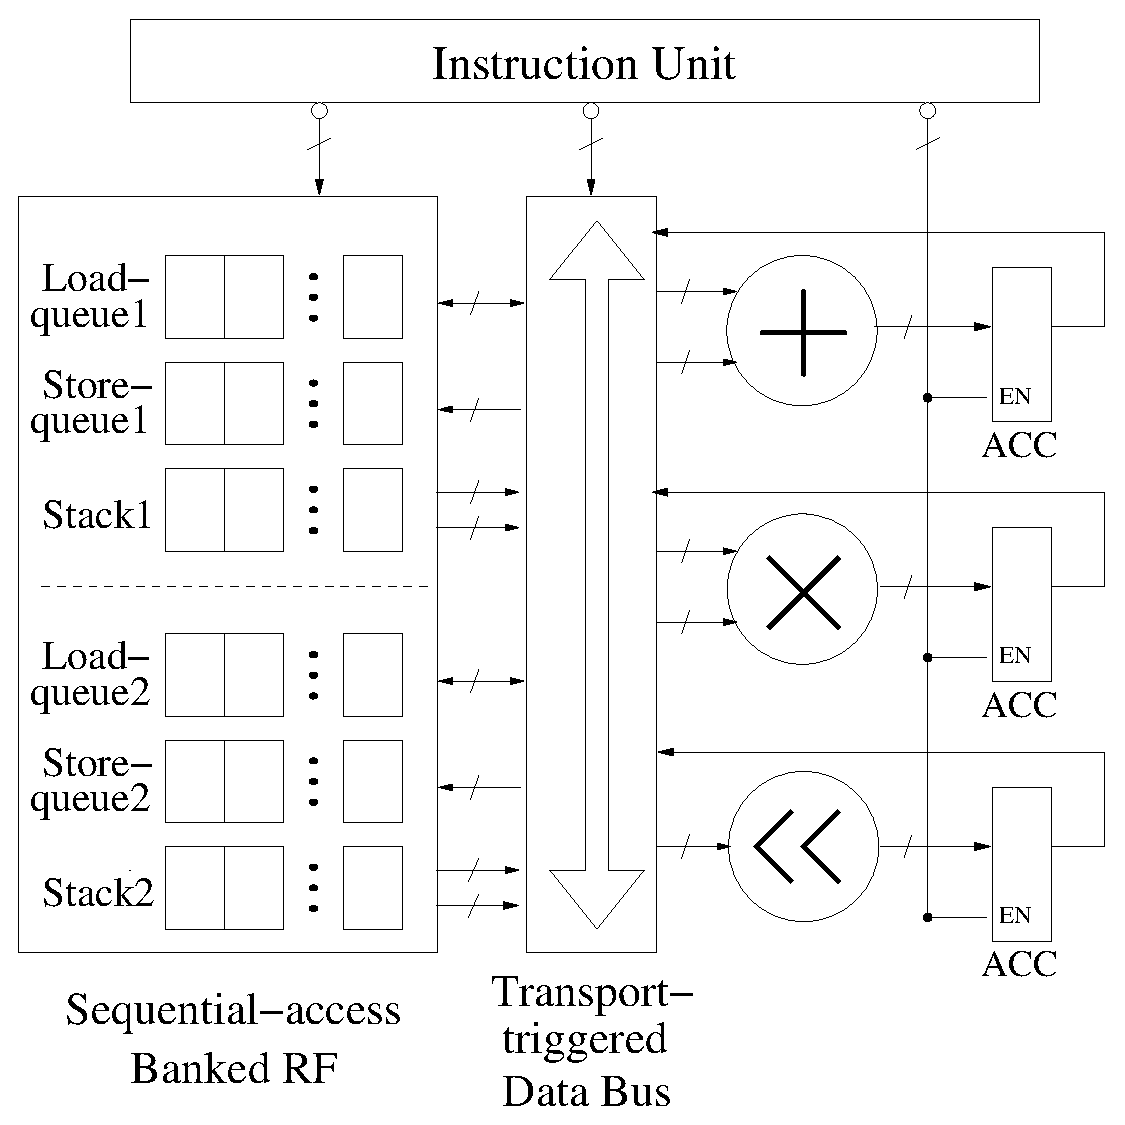
\includegraphics[width=0.85\textwidth]{./figs/micro.eps}
            \label{fig:micro}
        \end{figure}
    \section{Software Design}
            \label{sec:swdesign}
        \subsection{Software framework for DeAr}
            To fully exploit the power of DeAr, we also present a completed code generation flow including compilation, scheduling and optimization.
            Algorithm~\ref{alg:framework} provides an overview of the software framework for DeAr. 
            The user only need to provide DSP kernel code written in OpenCL and a flag which determines the optimization level as the input.
            With CLOC \cite{cloc} tool provided by \textit{HSA Foundation}, the kernel code is converted to standardized HSAIL, $H$, as shown in Line~\ref{line:tohsail}.
            Next, in Line~\ref{line:trans}-\ref{line:trane}, 
            we run the HSAIL transformation (elaborated in \ref{sec:trans}) on HSAIL code and obtain a hierarchical data flow graph (HDFG), 
            $\bar{G}$ (elaborated in \ref{sec:hdfg}), which holds crucial scheduling heuristics.
            After that, in Line~\ref{line:optstart} to \ref{line:optend}, we perform the key part of DeAr software, 
            operation scheduling and optimization (elaborated in \ref{sec:sando}).
            The optimization flag $\lambda$ in Line~\ref{line:forlambda} determines the number of iterations to be used.
            For each iteration, the scheduler exhausts heuristics in $\bar{G}$ which optimize the cycle and WB counts, 
            and it schedules operations with a limited randomness.
            Finally, the scheduler select the scheduling result with the least cycle count, 
            $C_{golden}$ among iterations and generates the final code $X_{golden}$ for DeAr as the output.
            %-----------------framework algo -------------
            \begin{algorithm}[h]
              \caption{\textproc{Software Framework for DeAr}}
              \begin{algorithmic}[1]
                    \Require 
                        High-level DSP kernel code in OpenCL, Optimization flag $\lambda$
                    \Ensure 
                        Binary code of DeAr

                  %\State Convert the kernel code to HSAIL code
                  \State $hsail \Leftarrow$ \Call{CL Offline Compiler }{ $kernel$ }
                  \label{line:tohsail}
                  %\State Perform SSA transformation on HSAIL;
                  %\label{tossa}
                  %\State Convert SSA code to DFG, $G = ( V_{op} , E_{op} )$, where $V_{op}$ is the set of operations and $E_{op}$ is the set of their dependencies;
                  %\label{todfg}
                  %\State Perform hierarchization on $G$, and get $\bar{G} = ( V_{bt} , E_{bt} )$, where $V_{bt}$ is a set of binary trees and $E_{bt}$ is the set of their dependencies;
                  \State $G \Leftarrow$ \Call{Convert HSAIL to DFG by SSA }{ $hsail$ }
                  \label{line:trans}
                  \State $\bar{G} \Leftarrow$ \Call{Hierarchize DFG to HDFG }{ $G$ }
                  %\State Perform the HSAIL transformation on HSIL code, and obtain a HDFG, $\bar{G}$
                  \label{line:trane}
                  \State $C_{golden} \Leftarrow  \infty$
                  \label{line:optstart}
                  \For {$i=1$ to $f(\lambda)$}
                    \label{line:forlambda}
                    %\State Schedule operations in $\bar{G}$ and get binary code $X_i$ and its total cycle count $C_i$
                    \State $X_{inter}, bt_{remain} \Leftarrow$ \Call{Inter-tree Scheduling }{ $\bar{G}$ }
                    \State $X_i, C_i \Leftarrow$ \Call{Intra-tree Scheduling }{ $X_{inter}, bt_{remain}$ }
                    \If {$C_i < C_{golden}$}
                      \State $C_{golden} \Leftarrow C_i$
                      \State $X_{golden} \Leftarrow X_i$
                    \EndIf
                  \EndFor
                  \State Return $X_{golden}$
                  \label{line:optend}
              \end{algorithmic}
              \label{alg:framework}
            \end{algorithm}
            %-----------------------------------------

        \subsection{Data Flow Graph and Hierarchical Data Flow Graph}
        \label{sec:hdfg}
            A data flow grahp (DFG), which presents dependencies among operations, is crutial information for program analysis.
            By partitioning a program into basic blocks, the control flow can be simplified, and thus each DFG of a basic block is a directed acyclic graph (DAG).
            Figure~\ref{fig:dfg:dfg} illustrates an example of a DFG, where each node and each edge denote an operation and a dependency respectively.
            We can further express any DFG as a data structure $G$, which holds a set of nodes (operations), $V_{op}$, and a set of edges (dependencies), $E_{op}$
            In conventional DSP software design, optimal scheduling of operations is often approached by analyzing DFGs.
            For example, \cite{dsplite} solves ILP problems \cite{ilp} in DFGs in scheduling, 
            and list scheduling \cite{list} calculates scheduling range of operations in DFGs as the scheduling criteria. 
            \\\indent
            However, we found that conventional DFG analysis is infeasible for scheduling in DeAr due to uniqueness of its datapath.
            As a result, in this work, we propose an enhanced version of DFG, hierarchical data flow graph (HDFG), to fit DeAr datapath.
            Figure~\ref{fig:dfg:hdfg} demonstrates an HDFG, $\bar{G} = {V_{bt}, E_{bt}}$, converted from Figure~\ref{fig:dfg:dfg}.
            We enumerate several important features of HDFG as below: 
            \begin{itemize}
                \item Cascaded operations, which implies no fork and join of edges within the cascade, are grouped into a super node ($sn$). 
                      If an operation is isolated, it forms a $sn$ directly.
                \item Neighboring $sn$ are further grouped into binary trees, $bt$s, which form a set of vertices, $V_{bt}$, in HDFG.
                      If a $sn$ is isolated, it forms a binary tree directly.
                \item Dependencies among operations that cross binary trees are inherited by binary trees they belong to.
                      These inherited dependencies form a set of edges, $E_{bt}$, among $V_{bt}$.
                \item A $bt$ without any in-edge existing in $V_{bt}$ (i.e., $\sum_{v \in V_{bt}}\textrm{deg}^-(bt) = 0$) is free to be scheduled. 
                      After scheduled, the $bt$ and its edge will be erased from $\bar{G}$.
                \item Every $sn$ must have either zero (leaf nodes) or two (non-leaf nodes) children.
                      Edges in a HDFG at $bt$, $sn$ and operation level guarantee the correctness of execution order.
            \end{itemize}
            \indent The hierarchy of HDFGs can provide crutial optimization heuristics to the DeAr scheduler.
            DeAr avoids RF access within each super node, and regularize RF access into first-in last-out fashion (stack) with the help from the recursive property of a binary tree.
            Moreover, the binary property also provides more opportunities to balance workload of two threads, and thus higher OPC can be achieved.
\begin{figure}[!ht]
    \begin{center}
    \subfigure[DFG example]
    {
        \label{fig:dfg:dfg}
        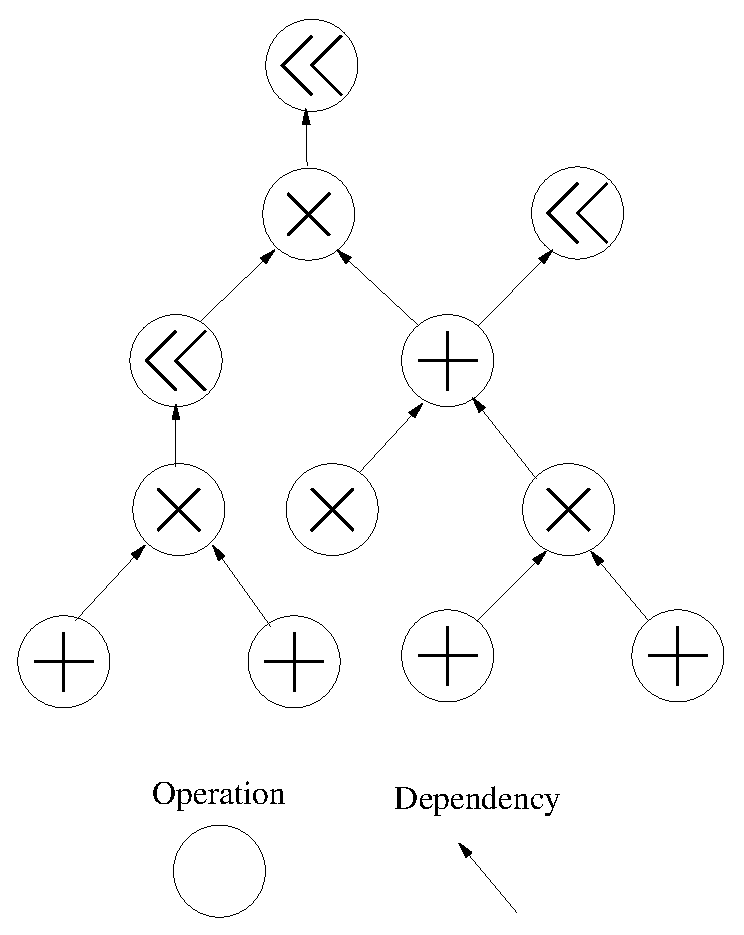
\includegraphics[width=0.45\textwidth]{figs/dfg.eps}
    }
    \subfigure[Corresponding HDFG]
    {
        \label{fig:dfg:hdfg}
        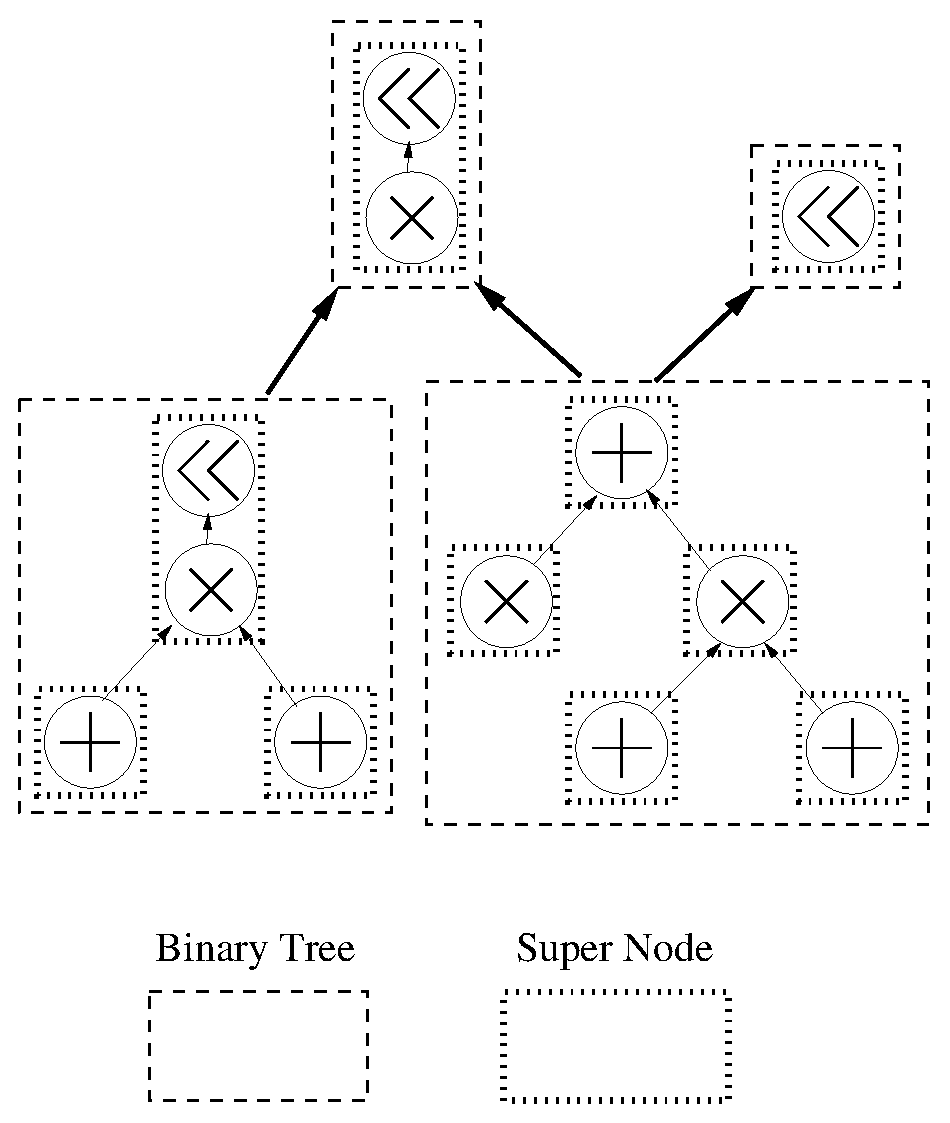
\includegraphics[width=0.45\textwidth]{figs/hdfg.eps}
    }
    \end{center}
    \caption{Conversion from DFG to HDFG}
    \label{fig:dfg}
\end{figure}

        
        \subsection{HSAIL Transformation}
        \label{sec:trans}
        The whole process of the HSAIL transformation contains two phases elaborated as below:
        \begin{itemize}
            \item \textbf{Phase 1: Convert HSAIL to DFG by SSA} \\\indent
                Algorithm~\ref{alg:2dfg} illustrates how this phase works.
                Single static assignment (SSA) \cite{ssa} is another form of IR which simplifies work of compiler significantly, 
                and thus deriving the SSA form of the code becomes the first step.
                SSA form specifies that each variable must be assigned exactly once, which is the key distinction from HSAIL.
                \\\indent
                The conversion from normal HSAIL to SSA form is initialized by performing reaching definition analysis \cite{rda} as shown in Line~\ref{line:rda}.
                Next, for each assignment in the code, we give a new name to the LHS variable, and update corresponding new names of RHS variables indicated by reaching definition analysis.
                These iterations which derive the SSA form correspond to Line~\ref{line:forhsails}-\ref{line:forhsaile}.
                Now, each assignment to some variable $X$ denotes an operation, which dominates operations with $X$ appearing in their RHS variables.
                As a result, we can construct the DFG without burden by iterating the new code, as shown in Line~\ref{line:forssas}-\ref{line:forssae}.
                Operations and their dependencies are stored in a set of vertices $V_{op}$ and a set of edges $E_{op}$ respectively, 
                and thus the DFG, $G = ( V_{op} , E_{op} )$, is constructed.
        %----------hsail to dfg algo--------------
        \begin{algorithm}[ht!]    \caption{\textproc{Convert HSAIL to DFG by SSA}}
        \begin{algorithmic}[1]
            \Require    HSAIL code
            \Ensure     $G = ( V_{op} , E_{op} )$   \Comment{ DFG }
            \State      Peform reaching definition analysis     \label{line:rda}
            \For        {each assignment (operation) in the HSAIL code}     \label{line:forhsails}
                \State      Give a new name to the LHS variable
                \State      Update RHS variables with corresponding new names in other assignments
                \EndFor                                                     \label{line:forhsaile}
            \State      Initialize $G \textrm{, where } V_{op} = \emptyset \textrm{ and } E_{op} = \emptyset $
            \For        {each assignment (operation) in the new HSAIL code} \label{line:forssas}    \Comment{SSA form}
                \State      Insert the LHS variable $x$ to $V_{op}$
                \For        {each variable $y$ in the RHS}
                    \State      Insert a new edge ($x$, $y$)
                \EndFor
            \EndFor                                                         \label{line:forssae}
        \end{algorithmic}
        \label{alg:2dfg}
        \end{algorithm}
        %----------------------------------------

            \item \textbf{Phase 2: Hierarchize DFG to HDFG} \\\indent
                As discussed in~\ref{sec:hdfg}, an HDFG is an enhanced version of a DFG which provides necessary heuristics for DeAr scheduler.
                Hierarchizing a DFG to an HDFG can be achieved by traversing the DFG, details of which are shown in Algorithm~\ref{alg:tohdfg}.
                In Line~\ref{line:forroots}-\ref{line:forroote}, the algorithm firstly iterates all root operations (i.e., $\textrm{deg}^+(op)=0$ ) in $G$,
                and call the first subroutine, \textproc{Build Binary Tree }, on each root operations.
                Line~\ref{line:bbts}-\ref{line:bbte} show the details of \textproc{Build Binary Tree }.
                A binary tree $bt$ is initialized by building a super node $sn$ on the input operation $op$ with the second subroutine, \textproc{Build Super Node }, 
                which groups cascaded operations ending with $op$, as shown in Line~\ref{line:bsns}-\ref{line:bsne}.
                After that, the third subroutine \textproc{Grow Binary Tree }, described in Line~\ref{line:gbts}-\ref{line:gbte}, will expand $bt$ by including neighboring operations if each of operations has exactly one out-edge (i.e., $\textrm{deg}^+(op)=1$), as shown in Line~\ref{line:growifs}-\ref{line:growife}. 
                \\\indent
                On the contrary, if the aforementioned condition is not met with any of $op_{left}, op_{right}$, 
                it will call \textproc{Build Binary Tree } on both to build new binary trees, $bt_{left}, bt_{right}$,
                and record the new dependencies, $bt_{left} \rightarrow bt, bt_{right} \rightarrow bt$.
                This step is demonstrated in Line~\ref{line:growelses}-\ref{line:growelsee}. 
                \\\indent
                The recursion proceeds by cross-calling between \textproc{Build Binary Tree } and \textproc{Grow Binary Tree } until the whole DFG is traversed.
                Binary trees and their dependencies are stored in a set vertices $V_{bt}$ and a set of edges $E_{bt}$ respectively.
                Finally, the HDFG, $\bar{G} = ( V_{bt} , E_{bt} )$, is constructed and returned.
        \end{itemize}

        %----------DFG to HDFG algo--------------
        \begin{algorithm}[ht!]    \caption{\textproc{Hierarchize DFG to HDFG}}
        \begin{algorithmic}[1]
            \Require    $G = ( V_{op} , E_{op} )$ \Comment{ DFG }
            \Ensure     $\bar{G} = ( V_{bt} , E_{bt} )$ \Comment{ HDFG }
            \State      Initialize $\bar{G} \textrm{, where } V_{bt} = \emptyset \textrm{ and } E_{bt} = \emptyset $
            \For        {each of $  op \ni \sum_{op \in V_{op}}\textrm{deg}^+(op) = 0 $}  \label{line:forroots}   \Comment{For each root vertex}
                \State      $v_{bt} \Leftarrow $\Call{Build Binary Tree }{$op$}
                \State      Insert $v_{bt}$ to $V_{bt}$
            \EndFor                                                                    \label{line:forroote}
            \Statex %---------------------------
            \Function   {Build Binary Tree }{$op$}         \label{line:bbts}
                \State      Initialize a birary tree $bt$
                \State      $sn \Leftarrow$ \Call{Build Super Node }{$op$}
                \State      Set $sn$ as the root of $bt$
                \State      \Call{Grow Binary Tree }{$sn$}
                \State      \Return {$bt$}
            \EndFunction                                \label{line:bbte}
            \Statex %--------------------------
            \Function   {Grow Binary Tree }{$sn$}          \label{line:gbts}
                \If         { $\textrm{deg}^-(sn.tail) = 2$ }     \Comment{A branch in the DFG}
                    \State      $op_{left}, op_{right} \Leftarrow op \ni (op \rightarrow sn.tail) \in E_{op}$ 
                    \If         {$\textrm{deg}^+(op_{left}) = \textrm{deg}^+(op_{right}) =1$}  \label{line:deg}  \label{line:growifs}
                        \State      $sn.left\_child \Leftarrow$ \Call{Build Super Node }{$op_{left}$}
                        \State      \Call{Grow Binary Tree }{$sn_{left}$}
                        \State      $sn.left\_child \Leftarrow$ \Call{Build Super Node }{$op_{right}$}
                        \State      \Call{Grow Binary Tree }{$sn_{right}$}     \label{line:growife}
                    \Else       \label{line:growelses}
                        \State      $bt_{new} \Leftarrow$ \Call{Build Binary Tree }{$op_{left}$}
                        \State      Insert the new tree $bt_{new}$ to $V_{bt}$
                        \State      Insert the new edge $(bt_{new} \rightarrow v_{bt})$ to $bt$
                        \State      $bt_{new} \Leftarrow$ \Call{Build Binary Tree }{$op_{right}$}
                        \State      Insert the new tree $bt_{new}$ to $V_{bt}$
                        \State      Insert the new edge $(bt_{new} \rightarrow v_{bt})$ to $bt$ \label{line:growelsee}
                        \EndIf                          \label{line:gbte}
                \EndIf
            \EndFunction
            \Statex %-----------------------
            \Function   {Build Super Node }{$op$}  \label{line:bsns}
                \State  Initialize a super node $sn$ 
                \State  $sn.head \Leftarrow op$
                \While{$\textrm{deg}^-(op) = 1$}
                    \State   $op \Leftarrow op_{next} \ni (op_{next} \rightarrow op) \in E_{op}$ 
                \EndWhile
                \State  $sn.tail \Leftarrow op$
                \State      \Return {$sn$}
            \EndFunction                        \label{line:bsne}
        \end{algorithmic}
        \label{alg:tohdfg}
        \end{algorithm}
        %--------------------------------------

    
        \subsection{Scheduling}

        A scheduler is responsible for ensuring the order of operations, 
        arranging data movement and allocating hardware resources.
        Once the scheduling result is determined, the corresponding machine code is also generated.
        The principle of the DeAr scheduler is, 
        two threads process binary trees in a HDFG concurrently and collaboratively until all operations are scheduled.
        Before exploring how threads co-work, we need to look into how a binary tree, $bt$, is handled by the scheduler.
        Algorithm~\ref{alg:sbt}, \textproc{Schedule Binary Tree}, 
        demonstrates how operaions of a $bt$ are scheduled into a specific sequence.
        %-------Schedule Binary Tree----------
\begin{algorithm}[!ht]
    \caption{\textproc{Schedule Binary Tree }}
    \begin{algorithmic}[1]
        \Require    $sn$
        \Ensure     $list_{op}$
        \If{$sn$ is NOT a leaf node}        \label{line:sbts}
            \State $size_{left} \Leftarrow$ \Call{Stack Size }{$sn.left\_child$}
            \State $size_{right} \Leftarrow$ \Call{Stack Size }{$sn.right\_child$}
            \If{$size_{left} > size_{right}$}
                \State \Call{Schedule Binary Tree }{$sn.left\_child$}
            \Else
                \State \Call{Schedule Binary Tree }{$sn.right\_child$}
            \EndIf
        \EndIf
        \State \Call{Schedule Super Node }{$sn$}   
        \State Erase $sn$ from the binary tree
        \If{$sn$ IS a root node}        
            \State \Return{$list_{op}$}
        \EndIf

        \label{line:sbte}
        \Statex
    \Function   {Stack Size }{$sn$}  \label{line:gsss}
        \If{$sn$ is a leaf node}
            \State $size \Leftarrow 0$
        \Else
            \State $size \Leftarrow \text{\textproc{Max}(\ \textproc{Stack Size }($sn.left\_child$), \textproc{Stack Size }($sn.right\_child$)\ )} + 1$
        \EndIf
        \State \Return{$size$}
    \EndFunction                    \label{line:gsse}
    \Statex
    \Function   {Schedule Super Node }{$sn$}  \label{line:ssns}
       \State   $op \Leftarrow$ $sn.tail$
       \Do   
           \State Insert $op$ to $list_{op}$
           \State $op \Leftarrow op_{next}$
       \DoWhile{$op \neq sn.head$}
    \EndFunction                            \label{line:ssne}

    \end{algorithmic}
    \label{alg:sbt}
\end{algorithm}
    %----------------------------------------------
        It traverse a $bt$ recursively in a post-order fashion, which implies the root is touched first but scheduled last.
        The input is the root $sn$ of a $bt$, and then a list of operations, which indicates execution flow, is returned.
        Line~\ref{line:sbts}-\ref{line:sbte} is the main part of the algorithm.
        For a input $sn$, the existence of its children is checked at the beginning.
        If children exist, the same algorithm, \textproc{Schedule Binary Tree }, is applied to them and the recursion starts.
        The first subroutine, \textproc{Stack Size } shown in Line~\ref{line:gsss}-\ref{line:gsse}, determines the precedence of children.
        After the recursion, the second subroutine, 
        \textproc{Schedule Super Node} shown in Line~\ref{line:ssns}-\ref{line:ssne}, is applied to this $sn$, 
        By this subroutine, cascaded operations in the $sn$ are scheduled consecutively.
        \\\indent
        The key insight of Algorithm~\ref{alg:sbt} is, it optimizes RF access significantly with heuristics from HDFGs.
        Firstly, operations in a $sn$ are scheduled consecutively.
        With this policy, the forwarding mechanism in DeAr can be taken advantage, and unnecessary WB is can be avoided.
        Secondly, the scheduler always schedules the child which demands larger stack size earlier, 
        By this mean, the stack size used by a parent $sn$ is the smaller one of two children plus one, 
        so that we can ensure the cost on stack size is minimized and prevent RF from spilling.
        \\\indent
        We further introduce \textproc{Inter-tree scheduling} and \textproc{Intra-tree scheduling}, 
        both of which require Algorithm~\ref{alg:sbt}.
        A typical HDFG contains multiple $bt$.
        As a result, the DeAr scheduler perform \textproc{Inter-tree scheduling} if multiple $bt$ exist.
        Algorithm~\ref{alg:inter} illustrate the detail of \textproc{Inter-tree scheduling}, 
        where a HDFG, $\bar{G}$ is input, and binary code segment, 
        $X_{inter}$, accompanied with a remaining subtree, $bt_{remain}$, will be returned.
        %-----------Inter-tree-------------
\begin{algorithm}[ht!]
    \caption{\textproc{Inter-tree Scheduling}}
    \begin{algorithmic}[1]
        \Require    HDFG $\bar{G} = (V_{bt}, E_{bt})$
        \Ensure     Remaining subtree $bt_{remain}$, binary code segment $X_{inter}$
        \State $X_{inter} \Leftarrow NULL$       \Comment{Initialize $X_{inter}$}
        \While{$V_{bt} \neq \emptyset$} \label{line:interws}
            \If{$work\_queue_{thread1} = \emptyset$}
                \State Select a binary tree $bt \ni \sum_{bt \in V_{bt}}\textrm{deg}^-(bt) = 0$ randomly
                \State $list_{op} \Leftarrow$ \Call{Schedule Binary Tree }{$bt.root$}
                \State Push $list_{op}$ into $work\_queue_{thread1}$
                \State Erase $bt$ and its edges from $\bar{G}$
            \EndIf
            \If{$work\_queue_{thread2} = \emptyset$}
                \State Select a binary tree $bt \ni \sum_{bt \in V_{bt}}\textrm{deg}^-(bt) = 0$ randomly
                \State $list_{op} \Leftarrow$ \Call{Schedule Binary Tree }{$bt.root$}
                \State Push $list_{op}$ into $work\_queue_{thread2}$
                \State Erase $bt$ and its edges from $\bar{G}$
            \EndIf
            \State $X_{inter} \Leftarrow X_{inter} \oplus$ \Call{Gen Code by DP}{$work\_queue_{thread1}$, $work\_queue_{thread2}$} \label{line:intercon}
        \EndWhile \label{line:interwe}
        \If{$work\_queue_{thread1} \neq \emptyset$} \label{line:interis}
            \State $bt_{remain} \Leftarrow$ \Call{Restore Subtree from Queue }{$work\_queue_{thread1}$}
            \State Clear $work\_queue_{thread1}$
        \ElsIf{$work\_queue_{thread2} \neq \emptyset$}
            \State $bt_{remain} \Leftarrow$ \Call{Restore Subtree from Queue }{$work\_queue_{thread2}$}
            \State Clear $work\_queue_{thread2}$
        \Else
            \State $bt_{remain} \Leftarrow NULL$
        \EndIf \label{line:interie}
        \State \Return{$X_{inter}$, $bt_{remain}$}
    \end{algorithmic}
    \label{alg:inter}
\end{algorithm}
        %------------------------------------------
        Line~\ref{line:interws}-\ref{line:interwe} enclosed by a while loop, is the main part of \textproc{Inter-tree scheduling}.
        The scheduler performs several identical steps for thread~1 and thread~2 respectively.
        It firstly search the whole $\bar{G}$ and select a free $bt$ randomly.
        Such a selection preserves randomness for DeAr scheduler, 
        and a better scheduling result is possible to be achieved with more trials, as discussed in Algorithm~\ref{alg:framework}.
        Next, the scheduler checks whether the work-queue of a thread is empty.
        If it is empty, the scheduler processes the selected $bt$ with Algorithm~\ref{alg:sbt}, 
        and enqueue the returned $op_{list}$ to the work-queue of a thread.
        Here, a work-queue is data structure that holds the operation sequence that belongs to a thread.
        An operation is removed from a thread's work-queue once it is indeed dispatched to binary code.
        After above steps, two work-queue are filled, and the key of this algorithm, \textproc{Gen Code by DP}, is performed.
        This subroutine, \textproc{Gen Code by DP}, dispatches operations in two work-queues which execute concurrently to binary code, 
        and arbitrates for FU conflict by Dynamic Programming (DP) \cite{dp}.
        It then returns a new code segment concatenated by the current one, and ensures at least one work-queue is cleared.
        Here, as shown in Line~\ref{line:intercon}, we use the sigh, $\oplus$, to denote the operation of code concatenation.
        Repeat of the loop proceeds until all $bt$ in $\bar{G}$ are consumed.
        However, it is very likely that there is a work-queue where operations remaining at the last iteration.
        Line~\ref{line:interis}-\ref{line:interie} illustrate such a scenario.
        Since the resulting binary code is incomplete, 
        remaining operations are reverted to the part of their original binary tree by \textproc{Restore Subtree from Queue},
        and a remaining subtree, $bt_{remain}$, is returned.
        \\\indent 
        To deal with $bt_{remain}$ and obtain the remaining part of the binary code, 
        \textproc{Intra-tree Scheduling}, illustrated in Algorithm~\ref{alg:intra}, is applied.
        %----------------Intra-tree---------------
\begin{algorithm}[!ht]
    \caption{\textproc{Intra-tree Scheduling}}
    \begin{algorithmic}[1]
        \Require    Remaining subtree $bt_{remain}$, binary code segment $X_{inter}$
        \Ensure     Final binary code $X_{final}$
        \State $X_{tail}, X_{body} \Leftarrow NULL$
        \While{$bt_{remain} \neq \emptyset$}    \label{line:intra:ws}
            \State $list_{op} \Leftarrow$ \Call{Schedule Super Node }{$X_{remain}.root$}
            \State Push $list_{op}$ into $work\_queue_{thread1}$
            \State $X_{tail} \Leftarrow$ \Call{Gen Code }{$list_{op}$} $\oplus X_{tail}$
            \State Erase $X_{remain}.root$ and obtain two sub-trees, $sbt_{left}, sbt_{right}$
            \Statex
            \State $list_{op} \Leftarrow$ \Call{Schedule Binary Tree }{$sbt_{left}.root$}
            \State Push $list_{op}$ into $work\_queue_{thread1}$
            \State $list_{op} \Leftarrow$ \Call{Schedule Binary Tree }{$sbt_{right}.root$}
            \State Push $list_{op}$ into $work\_queue_{thread2}$
            \State $X_{body} \Leftarrow X_{body} \oplus$ \Call{Gen Code by DP }{$work\_queue_{thread1}$, $work\_queue_{thread2}$}
            \Statex
            \If{$work\_queue_{thread1} \neq \emptyset$}
                \State $bt_{remain} \Leftarrow$ \Call{Restore Subtree from Queue }{$work\_queue_{thread1}$}
                \State Clear $work\_queue_{thread1}$
            \ElsIf{$work\_queue_{thread2} \neq \emptyset$}
                \State $bt_{remain} \Leftarrow$ \Call{Restore Subtree from Queue }{$work\_queue_{thread2}$}
                \State Clear $work\_queue_{thread2}$
            \Else
                \State $bt_{remain} \Leftarrow NULL$
            \EndIf
        \EndWhile   \label{line:intra:we}
        \State $X_{final} \Leftarrow X_{inter} \oplus X_{body} \oplus X_{tail}$
        \State \Return{$X_{final}$}
    \end{algorithmic}
    \label{alg:intra}
\end{algorithm}
        %-------------------------------------------
        The principle of \textproc{Intra-tree Scheduling} is similar to the one of \textproc{Inter-tree Scheduling} ---
        using two threads to process two $bt$ concurrently and collaboratively.
        Line~\ref{line:intra:ws}-\ref{line:intra:we} demonstrate a while loop, 
        which generates binary code iteratively.
        A crucial strategy applied here is, partitioning $bt_{remain}$ into three parts:
        the root node, left and right subtrees.
        Since operations in the root can only be handled sequentially, 
        we can dispatch them directly with a single thread (thread 1), 
        and obtain a tail segment of binary code, $X_{tail}$.
        Next, by treating left and right subtrees as independent ones, 
        we schedule them into work-queues of two threads respectively with \textproc{Schedule Binary Tree},
        and call \textproc{Gen Code by DP} to obtain another segment of binary code, $X_{body}$.
        By above steps, $bt_{remain}$ keeps shrinking while $X_{body}$ and $X_{tail}$ keep accumulating,
        until all operations left in $bt_{remain}$ are dispatched.
        Finally, we concatenate $X_{inter}$ from \textproc{Inter-tree Scheduling}, $X_{body}$ as well as $X_{tail}$,
        and obtain the complete binary code $X_{final}$.
        \\\indent
        The key insight of Algorithm~\ref{alg:inter} and Algorithm~\ref{alg:intra} is, they take advantage of DP.
        DP is a powerful technique often used in optimization with sequence data \cite{dpseq}.
        Letting OPC be the criteria, DP determines which of two threads should stall its operation when FU conflict occurs.
        As a result, a sequence of arbitrations optimized for ILP within a certain search space (product of two work-queues length), can be achieved.
        Moreover, the proposed algorithms also make use of the characteristic of a binary tree. 
        Even if only one $bt$ exists in HDFG, 
        the scheduler can still balance the workload of two threads by extracting left and right subtrees from $bt$ beforehand.


